\documentclass{article}
\usepackage{setspace}
\doublespacing
\usepackage{tikz-feynman}
\usepackage{amsmath}
\newcommand{\dd}{\textrm{d}}
\author{Silas Grossberndt}
\title{Renormalization and Learning}
%\subtitle{Searching Feynman Diagram expansions to define renormalization procedures relevant to Bayes net inference}
\usepackage{amsfonts}
\usepackage{graphicx}
\begin{document}
\maketitle
\section*{Abstract}
\hspace{0.5 cm} The work presented in this project creates an agent to calculate scattering amplitudes and physical measurables in particle physics systems. This work uses A$^*$ search to find corrections to coupling constants and scattering amplitudes in super renormalizable theories, in two different renormalization procedures, each of which inform the search by way of constrains informing further searching. This work is specifically done on a Lagrangian corresponding to the data structure of a Bayes net, which can be connected in an approach outlined in the literature. This is a proof of concept of this approach and fits in attempts to use AI tools and Particle Physics tools to inform data simulation and explainable AI models.
\section{Introduction}
This work aims to just explore the connections between my field of study, particle physics and AI. I am doing this by finding the renomalization of a lagrangian through A$^*$ and CSP applications. This work is suggested by other work recently done into deep learning and energy model AI and modeling theses with renormalization procedures
\subsection{Explainable AI and Explainable Deep Learning}
Mehta and Schwab \cite{Mehta2014} along with Beny \cite{Beny2013} have shown that the for deep learning on a state that can be describe as having some energy based description of initial and final states that the behavior of the learning is the same as that going on when a field in particle physics is renormalized, for more details, please see presentation
\subsection{Feynman Diagrams}
A Feynman diagram is a pictorial representation of the interactions between series of fields. These fields may be excited, creating particles, and interact with each other in ways governed by the energy description of the system, much in the way that states in energy model AI are described so too are particle interactions. However, what Feynman diagrams represent is a numerical evaluating of those states into a probability amplitude, which then can be converted into a physical measurable, and further branching of Feynman diagrams provide modifications to lower level calculations wherein the additional particles cost the system energy to produce but give more detail, factorizing the space \cite{PS}
\subsection{Renormalization in Particle Physics}
Renormalization is an approach wherein, in order to hand the fact that many theories will blow up in the energy needed to produce particles at some scale, we introduce a set of parameters that give a space where the theory is valid, restricting out state space and, for certian categories of theories called renormalizable and super-renormalizable wherein the divergences are well controlled and correspond to physical realities of the system that tell us about how scales of the universe interact with each other and give structures not immediately apparent when we evolve those interactions along a these scales. 

\section{Problem Statement and Goals}
\hspace{0.5 cm} This work aims to answer the following problems: How does one go about systematically calculating the impact of renormalization on a field theory? How do different methods of renormalization connect to each other and what does that relationship look like?
Then, the next question from the justification above is how does that structure of renormalization in each method correspond to a Bayes Net?

\hspace{0.5 cm} As a consequence of the first two questions, I needed to also define a method of representation and analysis of the field theory in question. 
I do this by starting from a Lagrangian and then digesting it to get the rules for what possible expansions can be made, and defining a set of constraints to allow for calculation of scattering amplitudes without the need for hand implementation of conservation of momenta. 
Then, this first solution is fed into further questions and then modified and informed by later solutions as the system is deeply entangled \cite{PS}. 
It should also be noted that there is not any one standard for how to represent and calculate Feynman diagrams computationally  \cite{Harlander1999} \cite{2009} \cite{Hodeges1990} \cite{TODOROV1971} \cite{BILENKY1974} or how to approach the problem of renormalization, due to the freedom in the theory itself \cite{Myers1996}\cite{Hansenfratz2019}\cite{Bednayakov2016} \cite{Carfora2010} 
\cite{Fabinao2022} \cite{Binosi2020}\cite{Sonoda2021}\cite{Aharony2019} \cite{Alekseev2005}. 
\subsection{Scope of work}
\hspace{0.5 cm} With the above stated problem, there is a wide scope of work that can be done. 
To properly account for all the space would be a series of multiple months worth of works for each sub-problem, so to keep the project manageable, I have made some specific choices. 
I have chosen to focus on the issue of defining the renormalization and not on the direct connection to the Bayes net, leaving that for future work. 
Additionally, I have chosen to only focus on scalar fields, as the integration and propagators that are involved are more straight forward and do not involve the need to introduce a gauge symmetry, matrix representations, non-Abelian algebras or Grassmanian variables, but it is anticipated that all of these could be introduced with further work. 

\hspace{0.5 cm}On this note, the apparent freedom in the selection of Lagrangian is actually hiding a bit of subtlety. 
This system inherently assumes that the theory is super-renormalizable and calculates as such. The test Lagrangian and most scalar fields that fit within the parameters of the system would follow this requirement, and this tracks on using it as an approximation towards xAI because this assumption does impose that the energy of the system is well defined, a useful condition for energy based AI models.
Then, in terms of the actual calculations, I did have to make a few approximations and restrictions (see heuristic discussion), but most importantly, I limited to numerical analysis and worked in the context of zero external momenta for the renormalization, which is one of the standard models \cite{PS} \cite{2009} \cite{Aharony2019} \cite{Myers1996}. 
\section{Methods}
\subsection{Algorithm design: Control Flow Diagram}
\hspace{0.5 cm}The general idea of the algorithm is that each node is a diagram, and the value of a node is its contribution to the overall scattering amplitude. 
In order to approach this, we need to have a prioritization for which diagram to expand first, a calculation of the scattering amplitudes (which involves a set of constraints wherein all the momenta at the vertices must sum to 0 which is a natural choice for a CSP, however, this is having some trouble right now, see section 3.3), a definition of the completion state, and a update of effective field theory that feed back into the Feynman generator. 
These controls are shown in the Control flow diagram shown in figure \ref{fig:cf}.
\newpage
\begin{figure}[!h]
\begin{center}
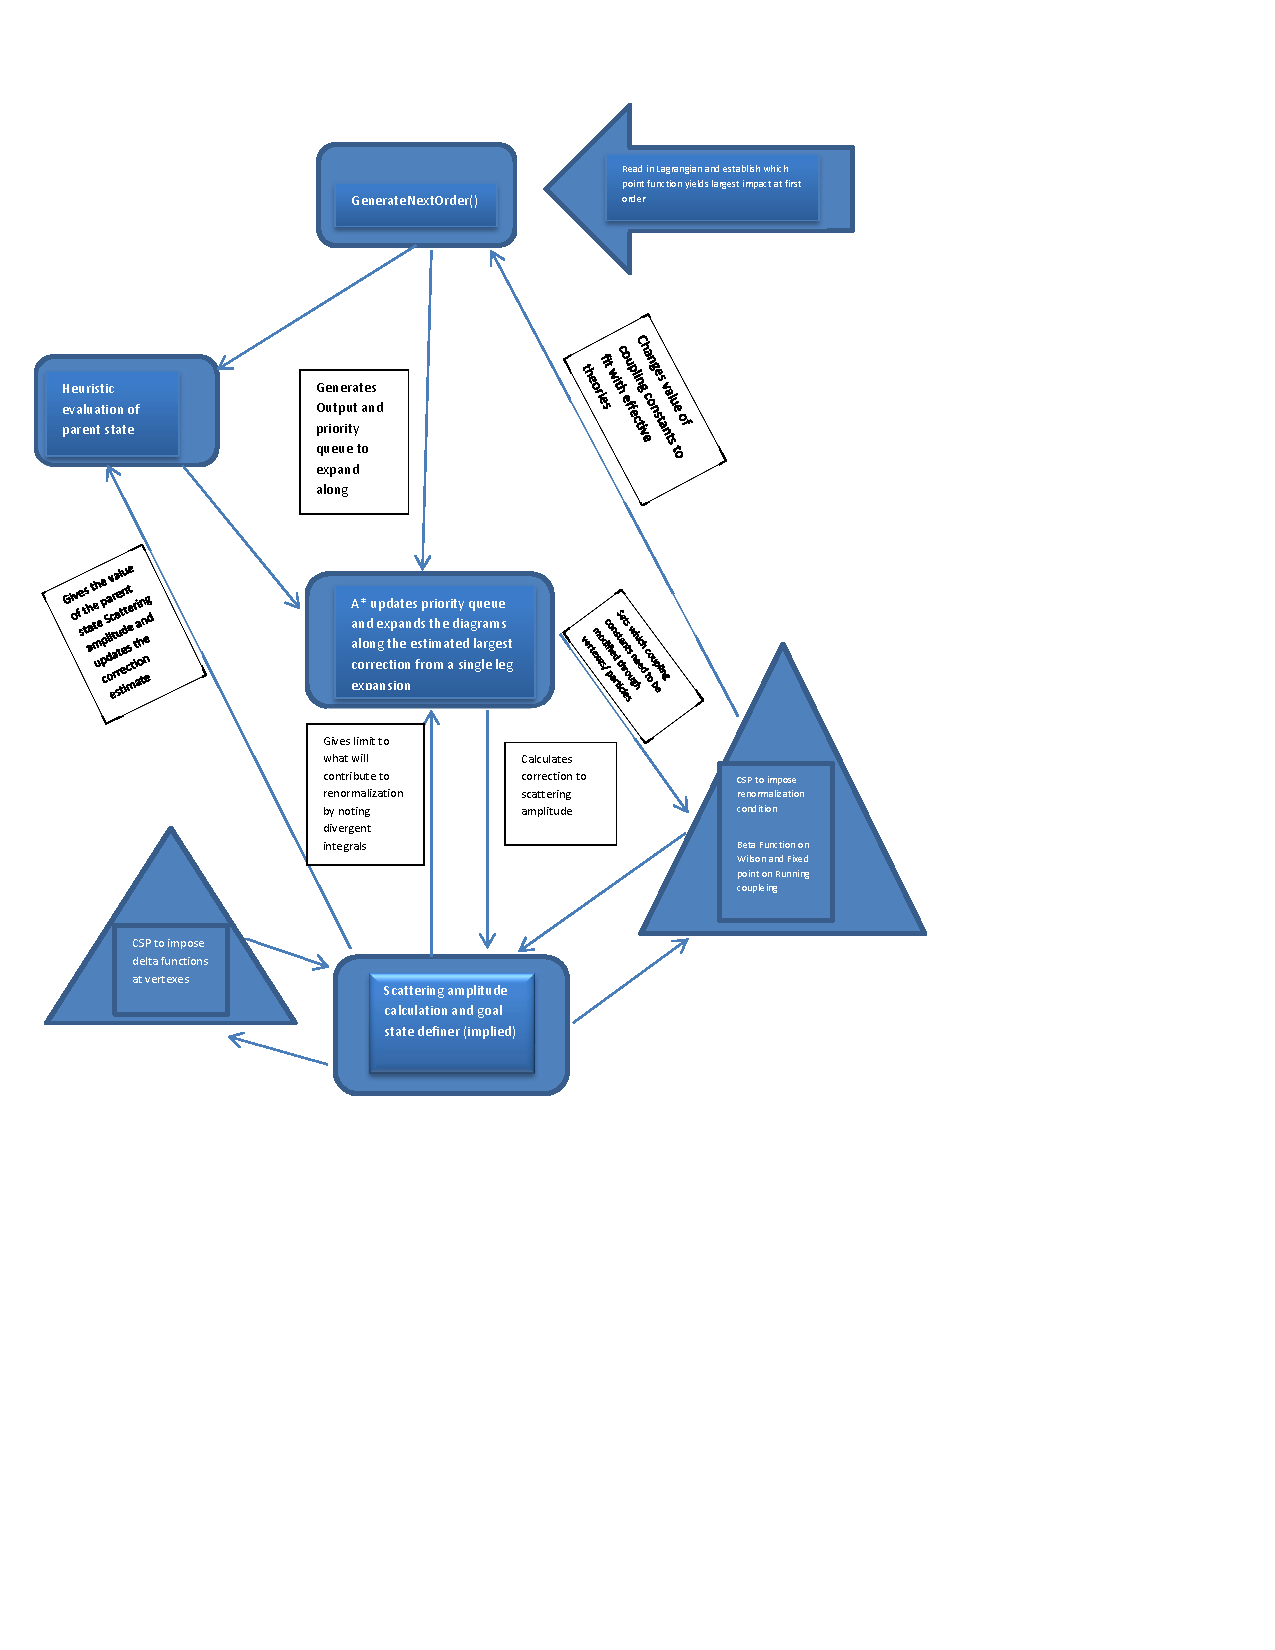
\includegraphics[ scale=0.8, trim={0  8cm 0 0}, clip]{Control_flow_diagram}
\label{fig:cf}
\caption{This gives the control flow for the A$^*$ search, wherein the priority queue in generated by optimizing impact on the scattering amplitude and the updating of the states then informs the generating of states further}
\end{center}
\end{figure}
\newpage
\subsection{Motivation for A$^*$ and why not LAO$^*$}
\hspace{0.5 cm}The key, for the nature of this class is the selection of the particular AI algorithms and why one would select one type over another. 
For this purpose, I knew that the idea was to find the path of diagrams that led to the optimal set of corrections to the scattering amplitude with out violation of renormalization conditions. These two requirements suggest immediately that some method of search is to be implemented, and that there are a set of constraints to be applied to the system. 

\hspace{0.5 cm} In terms of search, the state space is infinitely deep and is unlikely to have a terminating condition, so a depth first search would be deeply inappropriate as it could lead to infinite run times and never reaching a physically meaningful state. 
Then, the next choice to consider is a Breadth first search or a UCS. While these are both more useful than the depth first search, using either of these would raise the computational cost to go to any loop order, and lead to the calculation of irrelevant diagrams for the scattering amplitude, as not all Feynman diagrams at a particular loop order are going to give the largest contribution. 

\hspace{0.5 cm} Thus, one then lands on an A$^*$ approach. At first blush one notices that the recombination and expansion procedure detailed in section 3.4 would lead to the possibility of encountering acyclic graphs and entering a non-terminating state. To this end, I did consider implementation of the LAO$^*$ as detailed in \cite{Hansen}, however, ultimately I decided it was easier to implement A$^*$ with controlling the way expansion into child nodes would be handled, give that I was in charge of designing the data structure, thanks to the freedom allowed by the nature of perturbation theory, wherein I controlled for these potential issues in two ways. 
The first method was by casting out any doubling of any diagram and the second was through careful exploitation of graph symmetries (see section 3.4).
So by careful setting of definitions, I was able to force the state space into a tree, finding a simple path, as potential looping solutions could lead to runaway solutions, given that eh scattering amplitude would increase with each loop, giving a non-renormalizable theory, making it an appropriate approach for a theory like loop quantum gravity, wherein the graviton is a spin 2 particle that has a run-away divergence corresponding to a solution of a search with a loop, hence the name \cite{Bodendorfer2020} \cite{Jacobson2007}. Thus further, we can see the close connection between renormalization, particle physics and AI modeling, and immediately relevant research from this approach, enforcing the choice of a base algorithm of A$^*$ to expand from in further development.

\subsubsection{Heuristic}
\hspace{0.5 cm} I have selected the heuristic to be a proxy for the impact on the scattering amplitude, measured by the average over all possible vertex expansions on a node - the subtractive influence of the loop order. Then, I have subtracted the normalized form of that from 1 to build the priority queue so 
\begin{equation}
	h^* = \Delta SA/SA \hspace{1 cm} h= \frac{ \textrm{avg}\{\lambda_i\}}{SA * \sum m} -LO 
\end{equation}
	where this is guaranteed to be admissible. I got this through some back of the envelop calculations of the scattering amplitudes for 1 to 3 scalar fields up to loop 2. 
\subsection{Motivation for CSP}
\hspace{0.5 cm} In the course of creating this project I had initially planned on only using a CSP to give the change to the parameters of cutoff and effective coupling constants from the searching, however, when I was calculating higher loop order corrections, I realized that the integrals involved a set of constraints on internal momentum with one constraint per vertex. This involved imposing constraints while keeping free parameters, which previous methoods of perfoming the integration made impossible, being difficult to handle when dealing with a varied number of free parameters. The nature of a loop order is that it is defined as the number of free parameters that one must integrate over and then has a additional multiplicative integrand coming from the constraints. The number of constrained variables are 
\begin{equation}
	NC=I-L = I-(I-V+1)= V-1
\end{equation}
where $I$ is the number of internal lines and $V$ is the number of vertices or internal nodes of the graph. 
Then, given as this is a fluid constraint, as in any diagram of the same loop order may have a different set of functions defining the relations, but with a fixed family of constraints, the least intrusive calculation of these functions is through a CSP. This method worked well with smypy's integration functions that allowed for a more proper n-dimensional integral, however, I did use the assumption still that the transform to imaginary time could be justified, which while it does hold for this application and many others is not true in general. 

\hspace{0.5 cm}As for the CSP on the renormalization, this makes sense as it is really just a fixed point analysis, where in differential equations broadly define the interactions, but locally the constraint depends on evaluation of the state, giving a set of values that one can utilize and then enforce back on the state to inform better selection of future states. So while the first CSP was really a problem in its own right, this is more of an auxiliary function to the evaluation to the A$^*$
\subsection{Diagram representation and expansion}
\hspace{0.5 cm} The choice of diagram representation was helped by limiting to scalars. By limiting it to scalars, the directional of the lines did not matter so, the symmetry inherent in this reversibility allows for easier manipulation and restriction of the width of the state space, and prevents loops by identifying symmetric diagrams and imposing a multiplicative lowering corresponding to a symmetry factor on the scattering amplitude impact given by 
\begin{equation}
	\Sigma_{\textrm{vertexes}} \left( \begin{array}{c} k \\ n \end{array} \right)- (n-m) \min\{k, n-k\}  
\end{equation}
where the vertex has n many particles present, with k many on one side (either left or right) and with m many unique particles present. 

\hspace{0.5 cm} Then the expansion is done by taking a diagram, selecting one leg, and putting the possible vertices on that leg--called ``decorating'' in particle physics, and then recombining on exteriors to give diagrams of the same output.
\section{Running and Evaluation}
\subsection{Test Lagrangian and expected behavior}
\hspace{0.5 cm} The test condition for this system was run over the following Lagrangian
\begin{equation}
	\mathcal{L} = \frac{1}{2}\left( \partial_\mu \phi \partial^\mu \phi - m^2 \phi^2 + \partial_\mu \psi^* \partial^\mu \psi - M^2 \psi^* \psi \right) - \lambda \phi \psi^* \psi 
\end{equation}
which is the theory for two scalar fields, one real and one complex. This is a fairly standard collections of fields, chosen to meet with the structure of a learned Bayes net on the a burglary alarm dataset the structure of which is shown in figure 2, and is found in \cite[Morales2013], where the equivalence is found using the probability model outlined in \cite[JonaLasinio2001], working backwards to a theory that fits with the needed Renormalization Flow.
\begin{figure}[h!]
\begin{center}
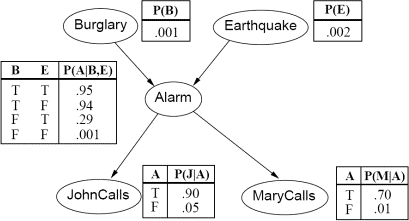
\includegraphics[scale=0.5]{EARTHQ}
\label{fig:eq}
\caption{The Bayes net structure that is aiming to be mimicked}
\end{center}
\end{figure}
This will give a renormalization where the coupling constant and cutoff (or scattering amplitude for the Willsonian approach) shift by the same amount then diverge, with one developing a new IR divergence corresponding to an inversion of the original UV divergence, so a $\log \Lambda$ goes to a $1/ \Lambda$ term
\subsubsection{ Running Coupling Renormalization Group Flow Equation}\
\hspace{0.5 cm} The renormalization for running coupling should go as 
\begin{equation}
	\frac{d \lambda}{d \Lambda} = 3 \lambda \log \Lambda
\end{equation}
and the local corrections are given as 	
\begin{equation}
	\Delta \lambda = - \frac{\Lambda \delta SA}{\delta \Lambda}
\end{equation}
with further constraint that the coupling constant must be always positive.
	
\subsubsection{Willsonian Renormalization}
\hspace{0.5 cm} The Willsonian approach doesn't change the cutoff but rather changes all possible coupling constants and limits changes on the scattering amplitude as 
\begin{equation}
 \frac{1}{\lambda'} - \frac{1}{\lambda} = \Delta SA \hspace{0.1 cm} \log \Lambda
 \end{equation}

\subsection{Evaluation}
The idea is that the renormalization will be run over all diagrams until the maximal change in the scattering amplitude is reached and the renormalization has reached the fixed point. 
Then, the two approaches will be compared using 
\begin{equation}
	\lambda_{RC} \frac{SA_{RC}}{\Lambda_{RC}} = \lambda_W SA_{W} \log( \Lambda_W)
	\end{equation}
	where $\Lambda_W$ is still the initial value which corresponds to a very energetic system, $p^2 +m^2 = 16 m^2$ so the internal particles may go up to very high energies, thus probing the smallest scale then coarse graining out to larger scales as was done in \cite{Beny2013} and \cite{Mehta2014}.
For this system the base diagram being expanded is
\begin{figure}[h!]
\begin{center}
\begin{tikzpicture}
\begin{feynman}
\vertex(i1) at (0,1);
\vertex(i2) at (1,1);
\vertex(o1) at (2, 2);
\vertex(o2) at (2,0);
\diagram{
	(i2)--[scalar, momentum=\( \phi \)](i1);
	(i2)--[scalar, momentum=\(\psi\)](o1);
	(i2)--[scalar, momentum=\(\psi^*\)](o2);
	};
	\end{feynman}
	\end{tikzpicture}
	\begin{tikzpicture}
\begin{feynman}
\vertex(i1) at (0,1);
\vertex(i2) at (1,1);
\vertex(o1) at (3, 2);
\vertex(a) at (2,2);
\vertex(b) at (2,0);
\vertex(o2) at (3,0);
\diagram{
	(i2)--[scalar, momentum=\( \phi \)](i1);
	(i2)--[scalar, momentum=\(\psi\)](a)--[scalar, momentum=\(\psi^*\)](o1);
	(i2)--[scalar, momentum=\(\psi^*\)](b)--[scalar, momentum=\(\psi\)](o2);
	(a)--[scalar, momentum=\(\phi\)](b);
	};
	\end{feynman}
	\end{tikzpicture}
	\caption{Vertex that we are expanding from, selected by analysis of ordering of vertex and maximum change to scattering amplitude and first expansion}
	\end{center}
\end{figure} 
\section{Results}
\hspace{0.5 cm} Having run over the set of all possible 3rd order diagram expansions and pointwise recombination, this has actually led to an interesting conundrum. Most of the interesting diagrams in this theory would be either computationally expensive to calculate or actually fail to rise past the $1\%$ contribution level, so the vast majority of diagrams must be skipped. 
Additionally, the use of the zero external momentum model allow for the state to be a vacuum expectation (i.e. particles being spontaneously crated from the vacuum) without causing a violation of conservation of energy and momentum.  
The simplicity of this model allows for calculation by hand of the first loop order contribution to the vertex is gotten by calculation of the integral \ref{eq:corr}
\begin{equation}
	-i \lambda^3 \int_0^\Lambda \frac{\dd^4 k}{(2\pi)^4} \frac{\dd^4 q}{(2 \pi)^4 }\frac{\dd^4 p}{(2 \pi)^4}\frac{1}{q^2 -m_{\psi}^2} \frac{1}{p^2-m_{\psi}^2} \frac{1}{k^2-m_{\phi}^2} (2\pi)^{12} \delta^4(p+q) \delta^4(p-k) \delta^4(k+q)  
\label{eq:corr}
\end{equation}
Evaluating this integral gives 
\begin{equation}
	\begin{split}
		\frac{\pi^2}{4(m_\psi^2 - m_\phi^2)^2(m_\psi^2 + \Lambda^2)} & \left[ (m_\psi^2 + \Lambda^2) \left( 2 m_\phi^3 \tan^{-1} \left( \frac{\Lambda}{m_\phi} \right) \right. \right. \\
		& \left. \left. + m_\psi (m_\psi^2 - 3 m_\phi^2 ) \tan^{-1} \left( \frac{\Lambda}{m_\psi} \right) \right) + m_\psi^2 \Lambda \left( m_\phi^2 - m_\psi^2 \right) \right] 
	\end{split}
\end{equation}
The output of running gives a number on this order (off by approximately $5\%$ a correction which is 
%This needs to have the stuff added to it, actually have results to add to this section finally. 
\newpage
\section{Further Work}
\subsection{Expanding the Theories}
\hspace{0.5 cm} This project presents a proof of concept of a renormalization performed on a simple construction of fields, particles and space, both to fit within the bounds of this project, and more broadly to fit within the bounds of computational intensity for a project of this nature that can be run locally on standard consumer hardware. Most similar projects, which are based on Monte Carlo approximation methods to give measurable results, tend to be far more computationally heavy. This comes down to a variety of concerns, chiefly the fact that the integrals involved become further convoluted and require integration over increasing degrees of freedom from higher symmetry representations. To this end, the version of the project presented here works solely with spin-less particles that interact only through the fundamental representation of a U(1) symmetry group, connected to a simple conservation law of total particle number. This theory is not particularly meaningful when it comes to real particles, however it does have interesting connections to the behavior of super-conductors and phonon theory. 
The next interesting connection to make would be to implement a simple electromagnetic theory of a photon and an electron with spin-dynamics. This system is well understood and is, in fact, one of the initial inspirations for the broad project of renormalization, however, the higher order corrections are still a subject of active research, and further implementation of heavier cousins of the electron (such as the muon) when considered in conjunction with other particle species is a subject of active debate specifically around how the charge and magnetic moment are to be interpreted in renormalization (see the recent controversy with the muon g-2 experiment at Fermi Lab). 
Ideally, I will mover this project to a C++ library and implement the full Standard Model Lagrangian as to allow for merging with other work on theorem proving and operator algebra approaches to renormalization. Other arenas of work include imposing more precise mathematical models of renormalization schemes--here I have presented the Minimal Subtraction scheme, however, this is just one of many potential procedures to follow--implementation of curved spaces, non-integer dimension, observable operators and twist expansions. 
The direct connection to the Bayes net has not been established in this work, and the general structure has been discussed, but fine tuning the parameters would still need to be implemented, which is a structure that would be nice to automate. Further computational tasks would naturally include a significant speed-up to allow for more intensive calculations, which would require dealing with memory usage, which at this point I have been allowing for python to automatically manage.
\subsection{Pitfalls and Limitations}
I have previously discussed future work of connecting this knowledge of renormalization group structure on the Bayes net using the technique used by Beny \cite{Beny2013}, and one would like to include a broader category of Lagrangians, allowing for spinor states to recreate solutions on the Ising glass model that has become a hallmark of this field, as well as introduce a GUI to the system to allow for us to truly make it user friendly and expand it out to broader use in both physics and AI communities. 
However, as it stands right now, I do have doubts about veracity of some of the approximations I made and I do think that my recombination and expansion routines may have been missing significant areas of use that would make further study impossible with the system in its current configuration. I also worry that without proper controls added, this system will fail if given a massless theory which is a standard test theory in particle physics, which would suggest that I should try to reestablish exactly how the external momenta impact the internal lines. This would require creative use of external constraints and spinor fields would allow this system to expand beyond the issue that a massless, spinless particle with zero momentum would lead to a $\frac{1}{0}$ integration, which is a physical result known in the literature as the infrared divergence that could be additionally integrated out by use of a lower bound renormalization as well as the upper bound approach presented here
\bibliographystyle{ieeetr}
\bibliography{XAI_renorm}
\end{document}
